\documentclass[UTF8]{article}
\usepackage{cite}
\usepackage[unicode,pdftex]{hyperref}
\usepackage{enumerate}
% \usepackage{geometry}
\usepackage{setspace}
\usepackage{pslatex} 
\usepackage{fancyhdr}
\usepackage{float}
\usepackage{amsmath}
\usepackage{titling}
\usepackage{indentfirst}
\usepackage{graphicx}
\usepackage{wrapfig}
\usepackage{amsmath}
\usepackage{xstring}
\usepackage{tikz}
\usetikzlibrary{fit, calc}
\pagestyle{empty} 



% \geometry{left=2.5cm, right=2.5cm, top=1.4cm, bottom=2.4cm}
\usepackage[a4paper,top=3cm,bottom=2cm,left=3cm,right=3cm,marginparwidth=1in, margin=1in]{geometry}
% \usepackage[margin=1in]{geometry}
\title{xxxxxxxxxxxxxxxxxxxxxxxx xxxxxxxxxxxxxxxxxxxxxxxx}
\author{Wenhao You(wyou1@ualberta.ca) Leo Chang(chewei@ualberta.ca)}
\date{}


\newcommand{\reffig}[1]{Fig. \ref{#1}}
\newcommand{\refsec}[1]{Section \ref{#1}}
% \newcommand{\refeq}[1]{Eq. \ref{#1}}
\newcommand{\reftab}[1]{Table \ref{#1}}


\fancyhead{}
\lhead{\scriptsize Chenqiu Zhao}
\rhead{\scriptsize research Proposal}

\renewcommand{\headrulewidth}{0pt}
\renewcommand{\normalsize}{\fontsize{12pt}{\baselineskip}\selectfont}


\newcommand{\chronoperiode}[7]{
	\pgfmathsetmacro{\first}{(#2 - 2018)*12 + #3 - .9} % beginig of the peropd
	\pgfmathsetmacro{\last}{(#4 - 2018)*12 + #5 - 1.1} % end of the period
	\pgfmathsetmacro{\middle}{(\first+\last)/2} % position of the country name
	\fill[#7] (\first,#6-1) rectangle (\last,#6) (\middle,#6-.5) node[white, font=\sf]{#1};
}

\definecolor{level1}{RGB}{200,10,20}
\definecolor{brightube}{rgb}{0.82, 0.62, 0.91}
\definecolor{fuchsia}{rgb}{1.0, 0.0, 1.0}
\definecolor{heliotrope}{rgb}{0.87, 0.45, 1.0}



\begin{document}
	\maketitle
	%\vspace{-90pt}
	
	
	
	
	
	
	\section*{Abstract}
	
	xxxxxxxxxxxxxxxxxxxxxxxx
	
	xxxxxxxxxxxxxxxxxxxxxxxx
	
	xxxxxxxxxxxxxxxxxxxxxxxx
	
	xxxxxxxxxxxxxxxxxxxxxxxx
	
	xxxxxxxxxxxxxxxxxxxxxxxx
	
	xxxxxxxxxxxxxxxxxxxxxxxx
	
	xxxxxxxxxxxxxxxxxxxxxxxx
	
	xxxxxxxxxxxxxxxxxxxxxxxx
	
	xxxxxxxxxxxxxxxxxxxxxxxx
	
	\section*{Introduction}
	
	%\begin{wrapfigure}{l}{0.5\textwidth}
	%  \vspace{-15pt}    % 对应高度1
	%  \includegraphics[width=0.5\textwidth]{figure/fig1.pdf}\\
	%   \label{fig1}
	%  \vspace{-15pt}    % 对应高度2
	% \caption{Deep distribution Learning for Background Subtraction.}
	% \label{fig1}
	%  \vspace{-15pt}    % 对应高度3
	% \end{wrapfigure}
Neural networks have been implemented on many applications and performed a great results. However, these neural networks are mostly implemented on a high-specification hardware such as computers since there are many parameters in different neural networks. The more parameters in the neural networks, the more storages and internet transmition rates are occupied. In this research, we try to look for a method that can make the neural networks run on a limited hardware devices, such as mobile devices. Although mobile devices have more enhanced hardware nowadays, but because of its limited size, the efficacy is still not as powerful as the computers. There are several benefits of running the neural networks on limited hardware devices, specifically, mobile devices. The most important part is the privacy and the data security. Processing data on-device ensures that personal information does not need to upload or transmit to the cloud servers, which enhanced privacy. 

Running neural networks on mobile devices can bring lots of advantages. Mobile devices, such as smartphones and tablets, play a significant role in our daily lives. If we are able to implement the neural network models directly on the mobile devices, it can reduce our dependence on the internet connection to some extent. Moreover, for some applications which need real-time feedback, such as object recognition and image segmentation, neural networks on mobile devices can also make the process faster and improve the user experience. The most important part of modern life is that we can keep the data processing and inference on our own interal system of the mobile devices rather than sending it to a remote server, which can enhance privacy and security to a great extent.

The new method called Frequency regularization (FR)~\cite{zhao2023frequency} is based on the frequency domain to compress the neural network. In this way, it can be divided into two steps: dynamic tail-truncation and inverse discrete cosine transform (IDCT). The main idea of this method is that some of the neural netwroks parameters may be redundant in their representation. The algorithm focus on using the frequency domain transform for network regularization to restrict information redundancy during the training process and introduce FR as shown in Fig.~\ref{idct}. Therefore, the redundant part can be removed without any side effect on the performance of the network.

\begin{wrapfigure}{l}{0.5\textwidth}
	\vspace{-15pt}    % 对应高度1
	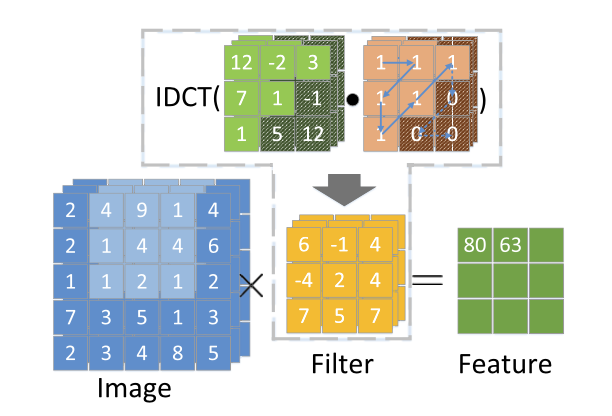
\includegraphics[width=0.5\textwidth]{figure/idct.png}\\
	\vspace{-15pt}    % 对应高度2
	\caption{Illustration of the proposed frequency regularization. The tail elements of tensors in the frequency domain are truncated first. then input into the inverse of the discrete cosine transform to reconstruct the spatial tensor for learning features~\cite{zhao2023frequency}.}
	\label{idct}
	\vspace{-15pt}    % 对应高度3
\end{wrapfigure}


In order to implement the neural networks on mobile devices, we have to think about the limitations of hardware and its characteristics. Many popular deep learning libraries, such as PyTorch and TensorFlow, are not complete and perfect to implement directly on the mobile devices. Thus, we need to edit some implementation in order to optimize specifically for the mobile devices such as TensorFlow Lite. By using the method, we can convert our standard neural network models into a lite format that can fit the mobile devices hardware better. Moreover, beyond this idea, we can also consider improving the hardware parts such as creating special neural network processors for the mobile. In this paper, we only explore the method in software instead of hardware.

Our paper makes discussion explores a simple, efficient, and creative method to transfer the large neural network into mobile devices, which is based on Frequency regularization. Our purpose is not only to accomplish this implementation but also to make sure the performance which should be the same as running on high-specification hardware such as computers. To sum up, we hope to provide a fast and secure neural network application experience for anyone who uses mobile devices.


% \begin{figure}[!h]
	%     \centering
	%     \includegraphics[width=0.5\textwidth]{../imgs/distribution.pdf}
	%     \caption{Segmenting moving objects in freely moving camera.}
	%     \label{fig_intro}
	% \end{figure}

\section*{Brief Summary of Existing Work}

xxxxxxxxxxxxxxxxxxxxxxxx

\subsection{Traditional Algorithms}
xxxxxxxxxxxxxxxxxxxxxxxx

xxxxxxxxxxxxxxxxxxxxxxxx

xxxxxxxxxxxxxxxxxxxxxxxx

xxxxxxxxxxxxxxxxxxxxxxxx

\subsection{Algorithms based on Machine Learning}
xxxxxxxxxxxxxxxxxxxxxxxx

xxxxxxxxxxxxxxxxxxxxxxxx

xxxxxxxxxxxxxxxxxxxxxxxx

xxxxxxxxxxxxxxxxxxxxxxxx

\subsection{Algorithms based on Deep Learning}
xxxxxxxxxxxxxxxxxxxxxxxx

xxxxxxxxxxxxxxxxxxxxxxxx

xxxxxxxxxxxxxxxxxxxxxxxx

xxxxxxxxxxxxxxxxxxxxxxxx

\section*{What you Plan To Do}
xxxxxxxxxxxxxxxxxxxxxxxx

xxxxxxxxxxxxxxxxxxxxxxxx

xxxxxxxxxxxxxxxxxxxxxxxx

\begin{itemize}
	\item Temporal Distribution Learning:
	Learn the distribution of temporal observations in a pixel, then classify if the pixel is foreground or background according to the distribution learned.
	\item Spatio-Temporal Distribution Learning:
	Incorporate the neighbouring information of pixels to improve the robustness and the efficiency of our background subtraction algorithm.
	\item Distribution Learning Layer:
	Devise a specific layer to learn the distribution.
	\item High Level Distribution Representation:
	Try to figure out what is the high level representation of distribution, what is the distribution of distribution.
	\item Deep Distribution Learning for General Problem:
	Extend the Deep Distribution Learning to other problems, instead of only used in background subtraction.
\end{itemize}

\section*{How You Plan to Implement Your Ideas}
xxxxxxxxxxxxxxxxxxxxxxxx

xxxxxxxxxxxxxxxxxxxxxxxx

xxxxxxxxxxxxxxxxxxxxxxxx


\section*{Timeline for Deep Distribution}

xxxxxxxxxxxxxxxxxxxxxxxx

xxxxxxxxxxxxxxxxxxxxxxxx

xxxxxxxxxxxxxxxxxxxxxxxx



\small
\bibliographystyle{unsrt}
% \bibliographystyle{plain}
\bibliography{ref.bib}  




\end{document}
